\section{Lab 3 - Complex Addition Systems}

\subsection{Introduction}
From your pocket calculator to inside modern CPUs adders have long been used as more than just a simple way to sum numbers together. This lab will go into the logic structure of the adder as well as provide a method for converting the simple full adder in to an \emph{arithmetic logic unit} (ALU) capable of handling 10 operations.

\subsection{Pre-lab}
Before coming to the lab, please complete the following and upload to Sakai:
\begin{itemize}
	\item A truth table for a half adder and a full adder
	\item The logic equation for a 4-bit ripple carry adder
\end{itemize}

\subsection{Lab Activities}

\subsubsection{Half Adder}
Build the circuit in Figure \ref{fig:halfadder}, create a test bench and verify that the logic is correct.

\begin{figure}[H]
	\centering
	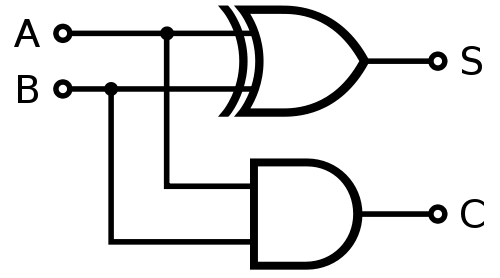
\includegraphics[width=60mm]{Lab3/figures/halfadder.png}
	\caption{Circuit for a 1-bit half adder}
	\label{fig:halfadder}
\end{figure}

\subsubsection{Full Adder}
The circuit in Figure \ref{fig:fulladder} implements a full 1-bit adder. Implement this circuit in VHDL, create a test bench, and verify that the logic behaves as expected. 

\begin{figure}[H]
	\centering
	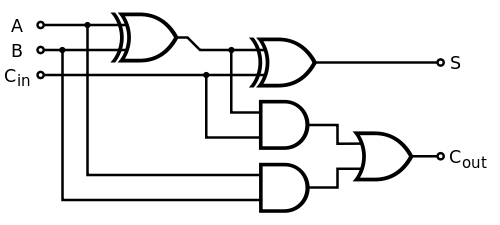
\includegraphics[width=80mm]{Lab3/figures/fulladder.png}
	\caption{Circuit for a 1-bit full adder}
	\label{fig:fulladder}
\end{figure}

Now that you have a working 1-bit full adder, implement a 4-bit ripple carry adder that sums the binary numbers "0110" and "0101." A block diagram for the 4-bit ripple carry adder is shown in Figure \ref{fig:fourbitripple}. Verify your results by creating a test bench and simulating the circuit.

\begin{figure}[H]
	\centering
	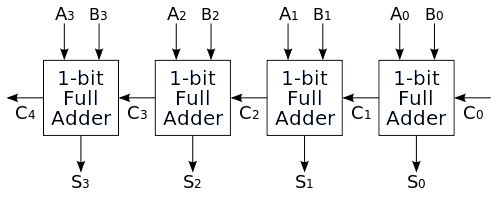
\includegraphics[width=100mm]{Lab3/figures/fourbitripple.png}
	\caption{4-bit ripple carry adder block diagram}
	\label{fig:fourbitripple}
\end{figure}

\subsubsection{Full Adder Based ALU}
The block diagram in Figure \ref{fig:fulladderalu} is an example of how the regular 1-bit full adder can be manipulated to implement additional functionality. For this activity, you must build VHDL code that implements a 4-bit complex adder ALU, the list of instructions can be found in Table \ref{tab:adderaluop}.

\begin{figure}[H]
	\centering
	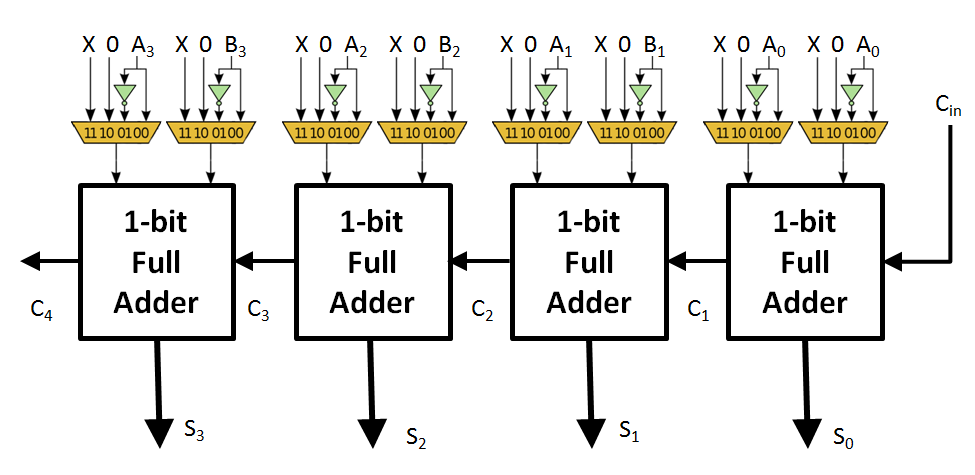
\includegraphics[width=150mm]{Lab3/figures/fulladderalu.png}
	\caption{Block diagram for a 4-bit ripple carry adder ALU with 10 operations}
	\label{fig:fulladderalu}
\end{figure}

After writing and testing your VHDL code, upload it on the DE2-115 FPGA Development board. Connect the inputs {\bf A3-A0} to SW3 - SW0 and the inputs {\bf B3-B0} to SW4(7)- SW(4). Also connect {\bf D$_1$} to SW(9) and {\bf D$_0$} to SW(8). Display inputs {\bf A} and {\bf B} in hexadecimal on HEX7 and HEX5, respectively and the output {\bf S} on HEX3. If the result over-flows display {\bf C$_4$} on LEDG0. If the result is negative turn on LEDR0 and if it is zero turn on LEDR1. Test and verify all ten operations and take a picture of each result (make a table that includes the values for {\bf A}, {\bf B}, {\bf S}, {\bf C$_4$}, {\bf Neg}, and {\bf Zero}.

\begin{table}[H]
	\centering
	\caption{List of opperations for the adder based ALU}
	\begin{tabular}{ | c | c | c | c | }
		\hline                        
 		\bf A$_i$ & \bf B$_i$ & \bf D$_0$ D$_1$ & \bf Result \\ \hline
 		Set to 0 & Set to 0 & 00 & 0 \\ \hline
 		Set to 0 &  Set to 0 &10 & 1 \\ \hline
 		A &  Set to 0 & 00 & A \\ \hline
 		Set to 0& B  & 00  & B  \\ \hline
 		A & Set to 0 & 10 & A $+$ 1 \\ \hline
 		Set to 0 & B & 10 & B $+$ 1 \\ \hline
 		A & B & 00 & A $+$ B \\ \hline
 		A & B & 10 & A $-$ B \\ \hline
 		Set to invert & Set to 0 & 01 & $\overline{A}$ \\ \hline
 		Set to invert & Set to 0 & 11 & $-$A \\ 
 		\hline
	\end{tabular}
	\label{tab:adderaluop}
\end{table}

When you finsih building the VHDL upload your code to the FPGA board. Test and verify all ten operations and take a picture of each result (make a table with that includes the values for {\bf A, B, S, C$_4$, Neg, and Zero}.

\subsection{Lab Report}
After completing the activities in this lab you should create a zip folder with the following and then submit it to Sakai:

\begin{itemize}
	\item Commented VHDL code.
	\item VHDL test benches for the half adder and full adder activities.
	\item Waveforms for the half adder and full adder activities.
	\item Pictures of the results from the ALU activity.
	\item A discussion on the results of compilation including longest path delay, the total number of logic elements used, and issues you encountered while performing the lab.
\end{itemize}

